\section{Telling waves from pull, and seeing in depth}\label{sec:separation}

\begin{quote}
\textbf{In plain words.} A wave from far away arrives at every pixel of the
camera almost identically, and so, nearly, does the pull of anything that is
not very close. What gives the wave away is its other half: a wave twists
spacetime as strongly as it stretches it, while still matter only stretches.
Nearby objects pull differently on different pixels, and those differences
tell how far away each thing is.
\end{quote}

Section~\ref{sec:pixel} ended with a difficulty: from the electric part alone,
one pixel cannot tell a wave from the pull of a passing lorry. With all ten
numbers it can (Section~\ref{sec:one-pixel}), and an array can do much more.
Three properties separate the two kinds of field.

\paragraph{Shape.} A plane wave stretches and squeezes only across its
direction of travel, so its tidal tensor has one vanishing eigenvalue and
$\det\tE = 0$. The field of a single mass has eigenvalues in the ratio
$-2 : 1 : 1$, and its determinant is never zero. One reading of one pixel
therefore distinguishes a single wave from a single mass. The test is for an
isolated source: the fields of several masses, or of several waves, add, and
their sum can have either form. The complex matrix of
Section~\ref{sec:one-pixel} goes further: a pure wave has
$\mathrm{tr}\,\mathcal{W}^2 = \mathrm{tr}\,\mathcal{W}^3 = 0$, two crossing waves have
$\det\mathcal{W} = 0$, and any single body has a repeated eigenvalue.

\paragraph{The magnetic part.} In a wave the magnetic tidal tensor is as large
as the electric one; it is the same pattern turned by $45^\circ$ about the
direction of travel. Near slowly moving matter it is smaller by the ratio of
the matter's speed to that of light,
\begin{equation}\label{eq:magnetic-ratio}
\frac{|\tB|}{|\tE|} = 1 \quad\text{(wave)},
\qquad
\frac{|\tB|}{|\tE|} \sim \frac{v}{c} \quad\text{(near field)} ,
\end{equation}
where $|\tE|^2 = \tE_{ij}\tE_{ij}$ (the Frobenius norm) and likewise for $\tB$,
and $v$ is the speed of the matter. At a distance $r$ from a compact source of
size $L$, the part of the field that changes is smaller by about $(v/c)(r/L)$,
that is, by $kr$ at the frequency of the change: more than $v/c$, but still far
below one in the near zone.
Averaged over time, the first holds for any mixture of waves from independent
sources, so the magnetic part is a detector of radiation that the pull of
nearby objects hardly touches. Coherent waves are an exception: in a standing
wave the magnetic part vanishes where the electric part is largest.

\paragraph{What the magnetic part sees nearby.} Small as it is, the near-field
magnetic tensor carries its own picture. To first order in $v/c$, a mass $M$ in
direction $\hat n$ at distance $r$, moving with velocity $\mathbf{v}$, gives
\begin{equation}\label{eq:magnetic-point}
\tB_{ij} = \frac{3GM}{c\,r^{3}}\,\bigl[\hat n_i(\hat n\times\mathbf{v})_j
+ \hat n_j(\hat n\times\mathbf{v})_i\bigr],
\end{equation}
which we have checked against the curvature of the metric of moving masses,
computed independently by finite differences. Grouping matter by direction
as in Eq.~\eqref{eq:tidal-column} gives the magnetic counterpart of the sky
integral,
\begin{equation}\label{eq:current-column}
\begin{gathered}
\tB_{ij} = \frac{3G}{c}\int\dd\Omega\,\bigl[\hat n_i(\hat n\times\mathbf{J})_j
+ \hat n_j(\hat n\times\mathbf{J})_i\bigr],\\
\mathbf{J}(\hat n) = \int \rho\,\mathbf{v}(r\hat n)\,\frac{\dd r}{r} ,
\end{gathered}
\end{equation}
so the magnetic half of the camera images the \emph{current column}
$\mathbf{J}$, with the same blur law at a signal-to-noise ratio smaller by
about $v/c$. Three things follow. Only motion across the line of sight counts:
$\hat n\times\mathbf{J}$ removes the radial part, so the magnetic channel is
the opposite of a Doppler radar, blind to approach and sensitive to sideways
motion. For a single moving mass $|\tB|/|\tE| = \sqrt3\,v_\perp/c$ to first order
in $v/c$, so one reading of one pixel gives the line on which a body lies (the
eigenvector of $\tE$'s negative eigenvalue, up to its sign) and, from $\tB$, its
sideways speed; at any speed, the four stars give the sideways velocity
exactly, Eq.~\eqref{eq:star-velocity}. And outside a spherical body spinning with angular momentum
$\mathbf{L}$ the field is exactly that of a spin dipole,
$\tB_{ij} = -(3G/cr^{4})[L_i\hat n_j + \hat n_iL_j
+ (\mathbf{L}\cdot\hat n)(\delta_{ij} - 5\hat n_i\hat n_j)]$: a hollow shell and
a solid ball of equal mass and size spinning at the same rate, whose electric
fields are identical everywhere outside them, differ in $\tB$ by their moments
of inertia, a factor $5/3$. At equal angular momentum they are identical
outside, and so motion too can hide. A uniform ball of radius $2^{-1/5}R$
turning one way inside a shell that reaches to $R$ and turns the other way at
the same rate has no angular momentum, and outside it no magnetic field at all,
though all of it moves; the reference implementation confirms the cancellation.
For a ball turning at angular velocity $\boldsymbol\omega$ about a point
$\mathbf{s}$, entered and left by the line of sight at distances $0 < a \le b$,
it is
$\mathbf{J} = \rho\,[(\boldsymbol\omega\times\hat n)(b-a)
- (\boldsymbol\omega\times\mathbf{s})\ln(b/a)]$. A smooth flywheel looks the
same spinning or still, and pulls the same; its current column is a vortex
that turns as the wheel turns. The demonstration of a sealed flywheel shows
it.

\paragraph{Variation across the array.} A wave of wavelength $\lambda$ changes
across an array of width $a$ by a fraction of order $2\pi a/\lambda$. The field
of a mass at distance $r$, which falls as $1/r^{3}$, changes by a fraction of
order $3a/r$. For a one-metre array, a wave at $100\,\mathrm{Hz}$ and a person
three metres away, these are $2\times10^{-6}$ and $1$. Subtracting the
average over the array therefore removes the wave and keeps the variation of
the neighbourhood. The reverse is harder: the average itself contains the pull
of everything nearby, and the person alone adds $3\times10^{-10}\,\mathrm{s^{-2}}$
to it, a million times the tidal field of the waves LIGO detects. To isolate
the wave the camera must model the nearby masses from their variation and
subtract them, which is how observatories plan to remove the changing pull of
their surroundings \cite{Harms2019,Chaibi2016}, or use the magnetic part, or
compare two arrays far apart; a camera simply keeps what the observatories
throw away. With two arrays far apart the separation is cleaner still: a wave
appears in both, with a delay that gives its direction, while a nearby mass
appears in one. The accompanying demonstrations show the tidal tensor itself
on a slice through the scene, coloured by the direction of stretching in the
manner of diffusion tensor imaging.

\paragraph{Depth.} The same variation measures distance. For an isolated mass
the tidal field goes as $M/r^{3}$ and its gradient as $M/r^{4}$, so their
ratio gives $r$, and then $M$: a pixel and its neighbours locate and weigh a
body with no need to move the camera. This is the principle by which a
calibration rotor's distance from a detector's mirror is found from the ratio
of two of its multipoles \cite{Inoue2018}. A single pixel can range a moving
mass without neighbours, but only with its magnetic part. The electric record
alone cannot do it: the record of a mass $M$ moving along $\mathbf{x}(t)$ is
unchanged if the path is enlarged $\lambda$-fold and the mass
$\lambda^3$-fold, while $\tB$ grows $\lambda$-fold, because the speed of light
supplies the scale. From Eq.~\eqref{eq:magnetic-point}, $\tB\hat n =
(3GM/cr^3)\,\hat n\times\mathbf v$ and $P\dot{\tE}\hat n = -(3GM/r^4)\,\mathbf
v_\perp$, with $P = 1 - \hat n\hat n$, so
\begin{equation}\label{eq:one-pixel-range}
r = c\,\frac{|\tB\hat n|}{|P\dot{\tE}\hat n|} ,
\end{equation}
and then $M$ from $\tE$; the sign that makes $r$ positive also fixes the sign
of $\hat n$. The reference implementation recovers distance, mass and velocity
this way from the finite-difference curvature of a moving mass. Motion straight
toward or away from the pixel gives no range, though it gives the time of
arrival, Eq.~\eqref{eq:contact}; and the magnetic signal, smaller by $v/c$, sets
the noise. For waves, range comes from the curvature of the wavefront, which
across an array of width $D$ amounts to a phase of order one at the distance
$D^{2}/\lambda$; beyond it range is still measured, with a fractional error of
order $\lambda r/\mathcal{R}D^{2}$ at signal-to-noise ratio $\mathcal{R}$. A
single pixel also ranges a wave source, from how its field departs from that of
a plane wave, Eq.~\eqref{eq:helicity-split}.

\paragraph{Front and back.} A flat array that records only the normal
component $\tE_{zz}$ cannot tell a mass in front of it from the mirror image of
that mass behind it, because the two give the same $\tE_{zz}$ on the plane. The
shear components $\tE_{xz}$ and $\tE_{yz}$ change sign between the two, so the
full tensor separates the half-spaces: a camera with no housing to block
gravity can still ignore the photographer standing behind it.

\paragraph{Three dimensions.} The pixels need not lie in a plane. A closed
shell of pixels sees the whole sky at once and has no blind side; pixels
filling a volume sample the field itself, although, as long as they stay
outside the matter, the ambiguity of Section~\ref{sec:near-field} remains. And in the thermal regime the transparency of matter makes a
further thing possible. Each image is then a set of line integrals, exactly
the data of a medical tomograph. Images from several positions can be combined
into a true three-dimensional map of emissivity, with nothing hidden behind
anything else.

These statements follow from the fields of
%   Sections~\ref{sec:pixel}--\ref{sec:waves}; the estimates of how well each
%   separation works in the presence of noise are still to be made.
% The text below begins with that paragraph's first sentence, kept. With it in place, the item "how well waves can
% be separated from nearby pull in the presence of noise, and the limits of the three-dimensional reconstructions of
% Section~\ref{sec:separation};" of paper/sections/12-status.tex is done, and the promise in the paragraph "How
% precisely" of paper/sections/02b-one-pixel.tex ("it ranges a moving mass with the precision that
% Section~\ref{sec:separation} gives") is kept by Eq.~\eqref{eq:magnetic-range}.
% References: three new entries in paper/drafts/separation_noise.bib (Ross2021, Thompson1982, Reid1990), to be added
% to paper/refs.bib. Figure: paper/figures/separation-noise.pdf, drawn by paper/figures/fig_separation_noise.py.
% Every number: reference/gravcam/separation_noise.py (paper_numbers), checked in
% reference/tests/test_separation_noise.py (test_numbers_quoted_in_the_draft and the tests above it).
% New labels: eq:magnetic-range, eq:depth-bound, fig:separation-noise.

These statements follow from the fields of
Sections~\ref{sec:pixel}--\ref{sec:waves}. How well each works against noise
follows from the Cram\'er--Rao bounds of the same fields, which the reference
implementation computes and checks against fits to simulated noisy readings
(Fig.~\ref{fig:separation-noise}). Each of a pixel's ten numbers carries white
noise, and $\rho$ is the signal-to-noise ratio of a signal at one pixel:
$|\mathcal{W}|/\sigma$ for one reading, as in Section~\ref{sec:one-pixel}, added
in quadrature over a record.

\paragraph{Separation with noise.} Take a wave at $100\,\mathrm{Hz}$ of strain
$10^{-21}$ and, $3\,\mathrm{m}$ from the camera, a rotor of two
$1\,\mathrm{kg}$ masses $12\,\mathrm{cm}$ apart turning 50 times a second,
about the quadrupole of the rotor that calibrates LIGO by its pull
\cite{Ross2021}. Its changing tide has the wave's frequency and a hundred times
its size. Shape alone tells an isolated wave from an isolated mass: the nearest
wave to the field of a mass, and the nearest mass to a wave, lie at half the
reading's size, so one reading of $\tE$ puts the two $\rho/2$ standard
deviations apart, and at $\rho = 12$ fewer than one reading in a hundred is
taken for the other. A wave and a near field together are separated by the
magnetic part, at a fixed price. Let the near field's $\tE$ at the wave's
frequency be anything at all, and its $\tB$ below the noise. Fitting both then
enlarges the error of the wave's amplitude by exactly $\sqrt2$, however strong
the near field: the near field takes the wave's $\tE$, and the wave is read from
its $\tB$, which carries half its signal. The wave is seen at $\rho/\sqrt2$, and
the near field pays the same $\sqrt2$ in the two components it shares with the
wave and nothing in the other three. Ignored, the rotor would be read as a wave
35 times the true one. Its own magnetic part leaks less than $10^{-4}$ of the
wave, because the $\tB$ of a changing source in the near zone is smaller than
its $\tE$ by a factor of order $kr$, here $2\times10^{-6}$, not by $v/c$. An
array that reads only $\tE$ must instead model the rotor from its variation,
here as a point quadrupole of unknown moment and position. For a pixel and six
neighbours at distance $b$ along three axes, the cost $D$, the factor on the
wave's error, grows as $r/b$, because a quadrupole's tide falls as $r^{-5}$ and
its share of the centre's reading must be inferred from a variation smaller by
about $5b/r$. For $b \ll r$, $D$ lies between $0.22\,r/b$ and $0.55\,r/b$ over
orientations. For the rotor and an array one metre across, $b = 0.5\,\mathrm{m}$,
$D = 2.2$; the array overtakes the magnetic part beyond $b = 0.29\,r$, and with
both $D = 1.26$. In return the wave costs the rotor's moment and position
factors of 1.5 and 1.3 from $\tE$ alone, and 1.07 and 1.04 with $\tB$ too.
Modelling the rotor as a point leaves a false wave of $0.005$ of the true one,
from its next multipole, which matters only above $\rho \approx 270$; ignored,
the rotor would be read as 70 times the wave.

\paragraph{How well depth is measured.} For one mass the field and its gradient
give the range exactly, $r = \sqrt{15}\,|\tE|/|\nabla\tE|$ with norms over all
components, and the Cram\'er--Rao bounds on range and mass are
\begin{equation}\label{eq:depth-bound}
\Bigl(\frac{\sigma_r}{r}\Bigr)^2 = \frac{1}{\rho_E^2} + \frac{1}{\rho_G^2},
\qquad
\Bigl(\frac{\sigma_M}{M}\Bigr)^2 = \frac{16}{\rho_E^2} + \frac{9}{\rho_G^2},
\end{equation}
where $\rho_E$ and $\rho_G$ are the signal-to-noise ratios of the field and of
its gradient, whatever the direction. A pixel with six neighbours at distance
$b \ll r$ has $\rho_E = \sqrt7\,\rho$ and $\rho_G = \sqrt{30}\,\rho\,b/r$, so
$\sigma_r/r \approx r/(\sqrt{30}\,\rho b)$; wider, the curvature of the field
across the pixels helps further. For a person $3\,\mathrm{m}$ away and
neighbours $0.5\,\mathrm{m}$ out, $\sigma_r/r$ is between $0.90/\rho$ and
$1.08/\rho$, depending on direction, against $1.16/\rho$ from the closed form
(Fig.~\ref{fig:separation-noise}b). Both uses of the
variation rest on Euler's relation for a field homogeneous of degree $-N$ about
its source, $(\mathbf{x}_s - \mathbf{x})\cdot\nabla f = N f$, with $N = 3$ for
the tide of a mass and $5$ for a quadrupole, by which geophysicists find the
depth of buried sources from measured gradients \cite{Thompson1982,Reid1990}.
The magnetic part of one pixel, Eq.~\eqref{eq:one-pixel-range}, ranges a moving
mass with no neighbours to
\begin{equation}\label{eq:magnetic-range}
\frac{\sigma_r}{r} = \frac{1}{\rho_B} ,
\end{equation}
$\rho_B$ the signal-to-noise ratio of $\tB$ alone, $\sqrt3\,v_\perp/c$ times
that of $\tE$ in each reading: for a person walking at
$1.4\,\mathrm{m\,s^{-1}}$, $\sigma_r/r = 1.2\times10^{8}/\rho$, a hundred
million times worse than with neighbours. Depth along one line is the limit.
For bodies on one line through the pixel every derivative of $\tE$ there has the
pattern of a single mass, so field and gradient see one body at
$r_{\mathrm{eff}} = \sum_i M_i r_i^{-3} / \sum_i M_i r_i^{-4}$, weighted toward
the nearer: two equal masses $\Delta$ apart appear as one at
$r - \Delta^2/r$, and a rod of length $L$ pointing at the camera as a point
$L^2/3r$ nearer than its centre. The spread $s$ of the depths shows first in
the second derivatives, as a share $s^2/r^2$ of them, which the seven pixels
read to $1/\rho_H$, with $\rho_H$ between $8.1$ and $10.5$ times
$\rho\,(b/r)^2$ depending on direction. Two equal masses, $s = \Delta/2$, are
therefore told from one only when $\Delta > 2r/\rho_H^{1/2}$, between $0.62$
and $0.70$ times $(r^2/b)/\rho^{1/2}$: the square-root law that
Section~\ref{sec:near-field} found for masses side by side. A round body of any
size is a point, and its size is not measured at all.

\begin{figure*}
\centering
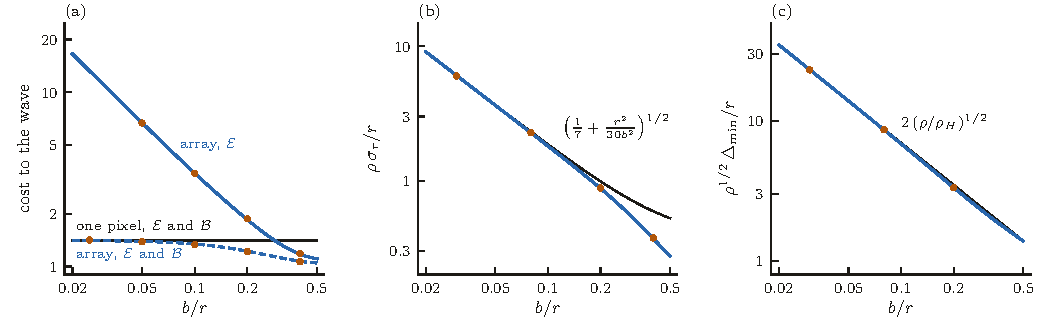
\includegraphics[width=\textwidth]{figures/separation-noise.pdf}
\caption{Separation and depth with noise, against the distance $b$ of a pixel's
six neighbours over the distance $r$ of the source. Blue: Cram\'er--Rao bounds
of the full models; black: closed forms; dots: the spread of
maximum-likelihood fits to simulated noisy readings. (a) The factor $D$ by
which fitting the rotor of the text enlarges the error of a wave's amplitude:
at one pixel from $\tE$ and $\tB$, with any near field, $\sqrt2$ (the dot at
left is a simulation with the rotor present); for the array, which fits the
rotor as a point quadrupole of unknown moment and position, from $\tE$ alone
(solid) and from both (dashed). (b) The range of one mass, with $\rho$ the
signal-to-noise ratio of one pixel's reading, against
Eq.~\eqref{eq:depth-bound}. (c) The separation $\Delta_{\min}$ in depth at which
two equal masses on one line are told from one at one standard deviation.
Computed in the reference implementation.}\label{fig:separation-noise}
\end{figure*}
